\documentclass[a4paper,twoside]{article}
% My LaTeX preamble file - by Nathaniel Dene Hoffman
% Credit for much of this goes to Olivier Pieters (https://olivierpieters.be/tags/latex)
% and Gilles Castel (https://castel.dev)
% There are still some things to be done:
% 1. Update math commands using mathtools package (remove ddfrac command and just override)
% 2. Maybe abbreviate \imath somehow?
% 3. Possibly format for margin notes and set new margin sizes
% First, some encoding packages and useful formatting
%--------------------------------------------------------------------------------------------
\usepackage{import}
\usepackage{pdfpages}
\usepackage{transparent}
\usepackage[l2tabu,orthodox]{nag}   % force newer (and safer) LaTeX commands
\usepackage[utf8]{inputenc}         % set character set to support some UTF-8
                                    %   (unicode). Do NOT use this with
                                    %   XeTeX/LuaTeX!
\usepackage[T1]{fontenc}
\usepackage[english]{babel}         % multi-language support
\usepackage{sectsty}                % allow redefinition of section command formatting
\usepackage{tabularx}               % more table options
\usepackage{booktabs}
\usepackage{titling}                % allow redefinition of title formatting
\usepackage{imakeidx}               % create and index of words
\usepackage{xcolor}                 % more colour options
\usepackage{enumitem}               % more list formatting options
\usepackage{tocloft}                % redefine table of contents, new list like objects
\usepackage{subfiles}               % allow for multifile documents

% Next, let's deal with the whitespaces and margins
%--------------------------------------------------------------------------------------------
\usepackage[centering,margin=1in]{geometry}
\setlength{\parindent}{0cm}
\setlength{\parskip}{2ex plus 0.5ex minus 0.2ex} % whitespace between paragraphs

% Redefine \maketitle command with nicer formatting
%--------------------------------------------------------------------------------------------
\pretitle{
  \begin{flushright}         % align text to right
    \fontsize{40}{60}        % set font size and whitespace
    \usefont{OT1}{phv}{b}{n} % change the font to bold (b), normally shaped (n)
                             %   Helvetica (phv)
    \selectfont              % force LaTeX to search for metric in its mapping
                             %   corresponding to the above font size definition
}
\posttitle{
  \par                       % end paragraph
  \end{flushright}           % end right align
  \vskip 0.5em               % add vertical spacing of 0.5em
}
\preauthor{
  \begin{flushright}
    \large                   % font size
    \lineskip 0.5em          % inter line spacing
    \usefont{OT1}{phv}{m}{n}
}
\postauthor{
  \par
  \end{flushright}
}
\predate{
  \begin{flushright}
  \large
  \lineskip 0.5em
  \usefont{OT1}{phv}{m}{n}
}
\postdate{
  \par
  \end{flushright}
}

% Mathematics Packages
\usepackage[Gray,squaren,thinqspace,cdot]{SIunits}      % elegant units
\usepackage{amsmath}                                    % extensive math options
\usepackage{amsfonts}                                   % special math fonts
\usepackage{mathtools}                                  % useful formatting commands
\usepackage{amsthm}                                     % useful commands for building theorem environments
\usepackage{amssymb}                                    % lots of special math symbols
\usepackage{mathrsfs}                                   % fancy scripts letters
\usepackage{cancel}                                     % cancel lines in math
\usepackage{esint}                                      % fancy integral symbols
\usepackage{relsize}                                    % make math things bigger or smaller
%\usepackage{bm}                                         % bold math!
\usepackage{slashed}

\newcommand\ddfrac[2]{\frac{\displaystyle #1}{\displaystyle #2}}    % elegant fraction formatting
\allowdisplaybreaks[1]                                              % allow align environments to break on pages

% Ensure numbering is section-specific
%--------------------------------------------------------------------------------------------
\numberwithin{equation}{section}
\numberwithin{figure}{section}
\numberwithin{table}{section}

% Citations, references, and annotations
%--------------------------------------------------------------------------------------------
\usepackage[small,bf,hang]{caption}        % captions
\usepackage{subcaption}                    % adds subfigure & subcaption
\usepackage{sidecap}                       % adds side captions
\usepackage{hyperref}                      % add hyperlinks to references
\usepackage[noabbrev,nameinlink]{cleveref} % better references than default \ref
\usepackage{autonum}                       % only number referenced equations
\usepackage{url}                           % urls
\usepackage{cite}                          % well formed numeric citations
% format hyperlinks
\colorlet{linkcolour}{black}
\colorlet{urlcolour}{blue}
\hypersetup{colorlinks=true,
            linkcolor=linkcolour,
            citecolor=linkcolour,
            urlcolor=urlcolour}

% Plotting and Figures
%--------------------------------------------------------------------------------------------
\usepackage{tikz}          % advanced vector graphics
\usepackage{pgfplots}      % data plotting
\usepackage{pgfplotstable} % table plotting
\usepackage{placeins}      % display floats in correct sections
\usepackage{graphicx}      % include external graphics
\usepackage{longtable}     % process long tables

% use most recent version of pgfplots
\pgfplotsset{compat=newest}

% Misc.
%--------------------------------------------------------------------------------------------
\usepackage{todonotes}  % add to do notes
\usepackage{epstopdf}   % process eps-images
\usepackage{float}      % floats
\usepackage{stmaryrd}   % some more nice symbols
\usepackage{emptypage}  % suppress page numbers on empty pages
\usepackage{multicol}   % use this for creating pages with multiple columns
\usepackage{etoolbox}   % adds tags for environment endings
\usepackage{tcolorbox}  % pretty colored boxes!


% Custom Commands
%--------------------------------------------------------------------------------------------
\newcommand\hr{\noindent\rule[0.5ex]{\linewidth}{0.5pt}}                % horizontal line
\newcommand\N{\ensuremath{\mathbb{N}}}                                  % blackboard set characters
\newcommand\R{\ensuremath{\mathbb{R}}}
\newcommand\Z{\ensuremath{\mathbb{Z}}}
\newcommand\Q{\ensuremath{\mathbb{Q}}}
%\newcommand\C{\ensuremath{\mathbb{C}}}
\renewcommand{\arraystretch}{1.2}                                       % More space between table rows (could be 1.3)
\newcommand{\Cov}{\mathrm{Cov}}
\newcommand\D{\mathrm{D}}
\newcommand*{\dbar}{\ensuremath{\text{\dj}}}

\newcommand{\incfig}[2][1]{%
    \def\svgwidth{#1\columnwidth}
    \import{./figures/}{#2.pdf_tex}
}

% Custom Environments
%--------------------------------------------------------------------------------------------
\newcommand{\lecture}[3]{\hr\\{\centering{\large\textsc{Lecture #1: #3}}\\#2\\}\hr\markboth{Lecture #1: #3}{\rightmark}}   % command to title lectures
\usepackage{mdframed}
\theoremstyle{plain}
\newmdtheoremenv[nobreak]{theorem}{Theorem}[section]
\newtheorem{corollary}{Corollary}[theorem]
\newtheorem{lemma}[theorem]{Lemma}
\theoremstyle{definition}
\newtheorem*{ex}{Example}
\newmdtheoremenv[nobreak]{definition}{Definition}[section]
\theoremstyle{remark}
\newtheorem*{remark}{Remark}
\newtheorem*{claim}{Claim}
\AtEndEnvironment{ex}{\null\hfill$\diamond$}%
% Note: A proof environment is already provided in the amsthm package
\tcbuselibrary{breakable}
\newenvironment{note}[1]{\begin{tcolorbox}[
    arc=0mm,
    colback=white,
    colframe=white!60!black,
    title=#1,
    fonttitle=\sffamily,
    breakable
]}{\end{tcolorbox}}
\newenvironment{problem}{\begin{tcolorbox}[
    arc=0mm,
    breakable,
    colback=white,
    colframe=black
]}{\end{tcolorbox}}

% Header and Footer
%--------------------------------------------------------------------------------------------
% set header and footer
\usepackage{fancyhdr}                       % header and footer
\pagestyle{fancy}                           % use package
\fancyhf{}
\fancyhead[LE,RO]{\textsl{\rightmark}}      % E for even (left pages), O for odd (right pages)
\fancyfoot[LE,RO]{\thepage}
\fancyfoot[LO,RE]{\textsl{\leftmark}}
\setlength{\headheight}{15pt}


% Physics
%--------------------------------------------------------------------------------------------
\usepackage[arrowdel]{physics}      % all the usual useful physics commands
\usepackage{feyn}                   % for drawing Feynman diagrams
%\usepackage{bohr}                   % for drawing Bohr diagrams
%\usepackage{tikz-feynman}
\usepackage{elements}               % for quickly referencing information of various elements
\usepackage{tensor}                 % for writing tensors and chemical symbols

% Finishing touches
%--------------------------------------------------------------------------------------------
\author{Nathaniel D. Hoffman}

\title{33-765 Homework 5}
\date{\today}
\begin{document}
\maketitle

\section*{16. Rare Event Statistics is Often Very Counter-intuitive}
The daily water height $ h $ at some coast line is a random variable. Let's assume it's distributed according to $ P_{\mu}(h) = \frac{4h}{\mu^2} e^{-2 h / \mu} $, with $ h \in \R^+ $. We are now concerned with building a levee that will keep people safe\textemdash with an acceptably low risk of failure.
\begin{itemize}
    \item[1.] Show that $ P_{\mu}(h) $ is normalized and that $ \ev{h} = \mu $. Plot $ P_{\mu}(h) $ (in suitably chosen units!\ Think!) as a function of $ h / \mu $.
        \begin{problem}
            \begin{align}
                \int_0^{\infty} P_{\mu}(h) &= \int_0^{\infty} \frac{4h}{\mu^2} e^{-2h / \mu} \dd{h} \\
                &= \frac{4}{\mu^2} \int_0^{\infty} h e^{-2h / \mu} \dd{h} \\
                u = - \frac{h}{\mu} \quad & \quad \dd{h} = - \mu \dd{u} \\
                &= 4 \int_0^{\infty } u e^{2u} \dd{u} \\
                &= 4 \left( \eval{\frac{ue^{2u}}{2}}_{0}^{\infty} - \int_0^{\infty} \frac{e^{2u}}{2} \dd{u} \right) \\
                v = 2u \quad & \quad \dd{u} = \frac{1}{2} \dd{v} \\
                &= 4 \left( \eval{\frac{ue^{2u}}{2}}_{0}^{\infty} - \frac{1}{4} \int_0^{\infty} e^v \dd{v} \right) \\
                &= \eval{\left[2 \frac{u e^{2u}}{2} - e^v\right]}_{0}^{\infty} \\
                &= \eval{- \frac{2h e^{- \frac{2h}{\mu}}}{\mu} - e^{- \frac{2h}{\mu}}}_{0}^{\infty} \\
                &= \eval{- \frac{(2h + \mu) e^{- \frac{2h}{\mu}}}{\mu}}_{0}^{\infty} \\
                &= 0 - \left( - \frac{\mu}{\mu} \right) = 1
            \end{align}
            Next, we want to show that $ \ev{h} = \mu $:
            \begin{align}
                \ev{h} &= \int_0^{\infty} \frac{4h^2}{\mu^2} e^{- \frac{2h}{\mu}} \dd{h} \\
                &= \frac{4}{\mu^2} \int h^2 e^{- \frac{2h}{\mu}} \dd{h} \\
                u = - \frac{h}{\mu} \quad & \quad \dd{h} = - \mu \dd{u} \\
                &= -4 \mu \int_0^{\infty} u^2 e^{2u} \dd{u} \\
                &= -4 \mu \eval{\left[ \frac{u^2 e^{2u}}{2} \right]}_{0}^{\infty} - \int u e^{2u} \dd{u} \\
                &= -4 \mu \eval{\left[ \frac{u^2 e^{2u}}{2} - \frac{u e^{2u}}{2} \right]}_{0}^{\infty} + \int \frac{e^{2u}}{2} \dd{u} \\
                &= \eval{\left[- \frac{2h^2 e^{- \frac{2h}{\mu}}}{\mu} - 2 h e^{- \frac{2h}{\mu}} - \mu e^{- \frac{2h}{\mu}}\right]}_{0}^{\infty} \\
                &= \eval{- \frac{(2 h^2 + 2 \mu h + \mu^2) e^{- \frac{2 h}{\mu}}}{\mu}}_{0}^{\infty} \\
                &= 0 - \left( - \frac{\mu^2}{\mu} \right) = \mu
            \end{align}
        \end{problem}
        \begin{figure}[h]
            \centering
            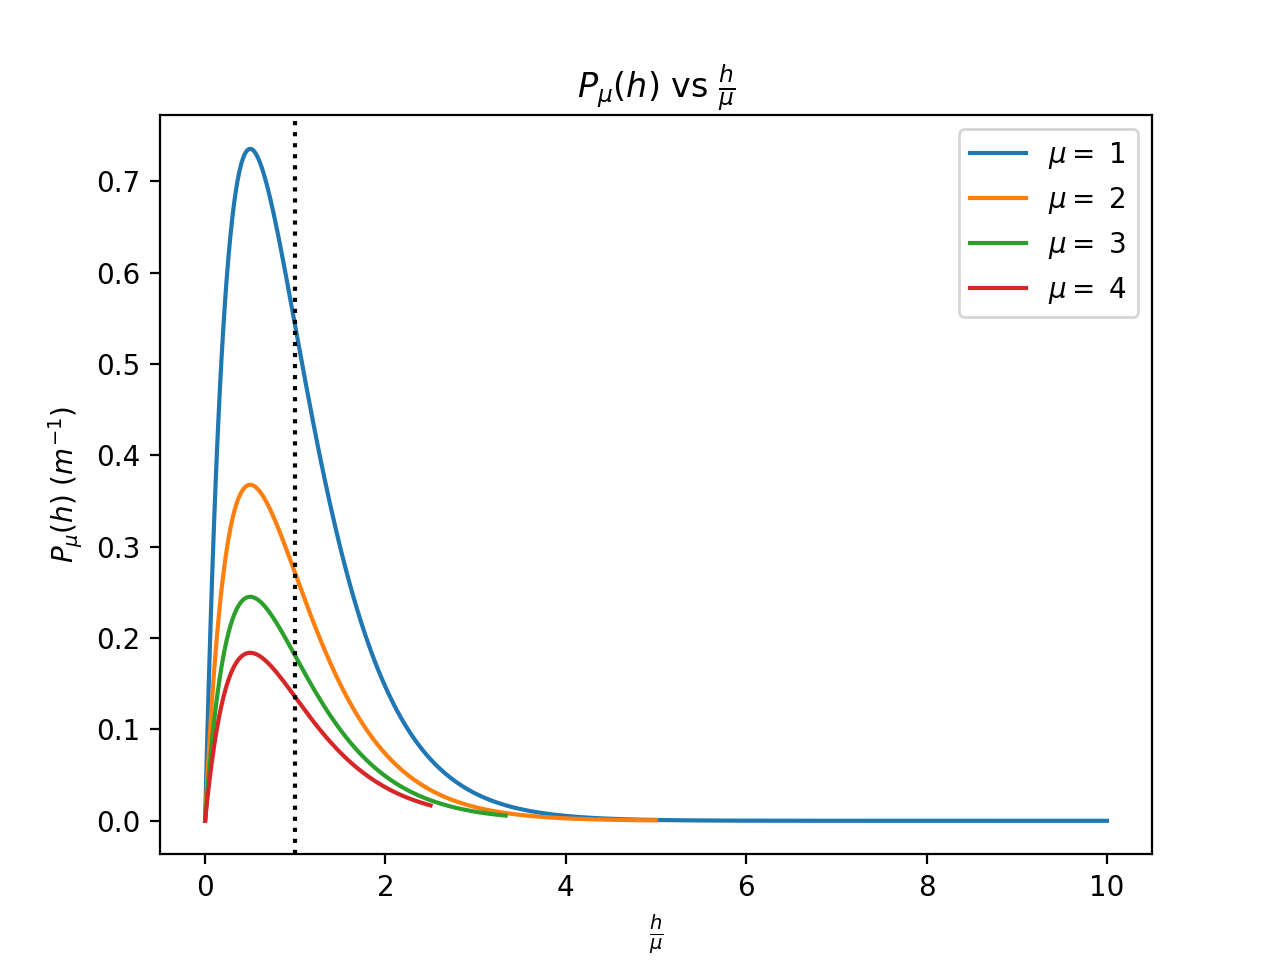
\includegraphics{Problem_16_Plot.png}
            \caption{Graph for Problem 16.1}
            \label{fig:graph_problem_16}
        \end{figure}
    \item[2.] Let's assume $ \mu = 1\meter $. How high do we have to build a levee such that the risk of it getting flooded is less than once every $ 500 $ years? You will arrive at a transcendental equation for the levee height $ L $, which you have to solve numerically.
        \begin{problem}
            The function given above corresponds to the probability that the water will be at height $ h $ on a given day given that the average height is $ \mu $. Therefore, we need to integrate this distribution from $ 0 $ to a value $ L $ such that the integral is equal to $ 1 - D $ where $ D = \frac{1\text{ day}}{ 500\text{years}} = \frac{1}{182,500} = 0.0000055$:
            \begin{equation}
                \int_0^L P_{\mu}(h) \dd{h} = 0.9999945 = 1 - \frac{2L + \mu}{\mu} e^{- \frac{2L}{\mu}}
            \end{equation}
            Solving this in Mathematica with $ \mu = 1 $, I find that
            \begin{equation}
                L = 7.437\meter
            \end{equation}
        \end{problem}
    \item[3.] Assume $ \mu $ increases by $ 20\centi\meter $ due to global warming. What's now the time scale on which the levee we built is flooded?
        \begin{problem}
            If we set $ L = 7.437 $ and $ \mu = 1.20 $, we can calculate the value of the integral and figure out how many days that corresponds to. The integral evaluates to $ 0.999945 $. Solving $ (1-0.999945) = \frac{1}{365*x} $ for $ x $ gives $ 50 $ years, which is surprisingly less than the $ 500 $ year mark we started with.
        \end{problem}
    \item[4.] By how much do we have to increase the height of the levee to get the flooding risk back to once every $ 500 $ years?
        \begin{problem}
            With $ \mu = 1.20 $, the new height of the levee (solving the same equation with Mathematica) is
            \begin{equation}
                L = 8.9253\meter
            \end{equation}
            which means we need to increase it by $ 1.49\meter $.
        \end{problem}
\end{itemize}

\section*{17. Closed Versus Exact Differentials\textemdash The Fine Difference}
Show that the differential $ \dbar{f} = \frac{-y \dd{x} + x \dd{y}}{x^2 + y^2} $ is closed but not exact. Why does this happen?
\begin{problem}
    If $ \dbar{f} = a \dd{x} + b \dd{y} $, then $ \pdv{a}{y} = \pdv{b}{x} $ means that the differential is closed. We can see that for this differential, $ a = \frac{-y}{x^2 + y^2} $ and $ b = \frac{x}{x^2 + y^2} $, so
    \begin{equation}
        \pdv{a}{y} = \frac{2y^2}{(x^2 + y^2)^2} - \frac{1}{x^2 + y^2} = \frac{y^2 - x^2}{(x^2 + y^2)^2}
    \end{equation}
    and
    \begin{equation}
        \pdv{b}{x} = - \frac{2 x^2}{(x^2 + y^2)^2} + \frac{1}{x^2 + y^2} = \frac{y^2 - x^2}{(x^2 + y^2)^2}
    \end{equation}
    so
    \begin{equation}
        \pdv{a}{y} =  \pdv{b}{x}
    \end{equation}
    However, a closed differential is only exact if its domain is simply connected. This means any simple closed curve in the domain can be continuously shrunk to a point in the set. However, this is not true for this differential, since the point $ (x=0, y=0) $ is undefined in this differential. We can also show this by showing that integrals around a closed curve about the origin will be nonzero. Specifically, if we transform to spherical coordinates, $ x = r \cos(\theta) $, $ y = r \sin(\theta) $, $ x^2 + y^2 = r $, $ \dd{x} = \cos(\theta) \dd{r} - r \sin(\theta) \dd{\theta} $, $ \dd{y} = \sin(\theta) \dd{r} + r \cos(\theta) d \theta $:
    \begin{equation}
        \dbar{f} = - \frac{\sin(\theta)}{r} \dd{x} + \frac{\cos(\theta)}{r} \dd{y} = \dd{\theta}
    \end{equation}
    Therefore, the integral around any closed simple curve around the origin will result in $ 2 \pi $ times the winding number of the curve, which cannot be zero.
\end{problem}

\section*{18. Maximum Work from a Temperature Difference}
Suppose we have two buckets of water with constant heat capacities $ C_A $ and $ C_B $, so that the relationship between the change of temperature in bucket $ i $ and its change in energy is $ \dd{U_i} = C_i \dd{T} $. The buckets are initially at temperature $ T_{A,0} $ and $ T_{B,0} $. We now put an ideal heat engine between these two buckets, depleting the temperature difference to extract mechanical work.
\begin{itemize}
    \item[1.] What is the final temperature of the water in the two buckets? \textit{Hint: Start by drawing a diagram of how you connect the buckets and the machine, show your flow of heat and work.}
        \begin{problem}
            First, because neither the volume of the buckets nor the number of particles in them are changing,
            \begin{equation}
                \dd{U} = T \dd{S}
            \end{equation}
            Therefore, the total change in entropy for each bucket will be
            \begin{equation}
                \dd{S_i} = \frac{\dd{U_i}}{T_i} = C_i \frac{\dd{T_i}}{T_i}
            \end{equation}
            The total change in entropy must be zero, so
            \begin{align}
                0 &= C_A \frac{\dd{T_A}}{T_A} + C_B \frac{\dd{T_B}}{T_B} \\
                &= C_A \dd{\ln(T_A)} + C_B \dd{\ln(T_B)} \\
                &= \dd{(\ln( (T_A)^{C_A} (T_B)^{C_B}))} = 0
            \end{align}
            so
            \begin{equation}
                (T_{A,0})^{C_A} (T_{B,0})^{C_B} = (T_{A,f})^{C_A} (T_{B,f})^{C_B}
            \end{equation}
            In the final state, the temperatures of the buckets must be equal, since that will be the point at which there is no more heat to extract as work. if $ T_{A,f} = T_{B,f} = T_f $, then
            \begin{equation}
                (T_{A,0})^{C_A} (T_{B,0})^{C_B} = (T_f)^{C_A + C_B}
            \end{equation}
            or
            \begin{equation}
                T_f = \left( (T_{A,0})^{C_A} (T_{B,0})^{C_B}\right)^{\frac{1}{C_A + C_B}}
            \end{equation}
        \end{problem}
    \item[2.] What is the maximum amount of work you can extract with such a heat engine from the two buckets?
        \begin{problem}
            The maximum work is equal to the heat transferred from both buckets:
            \begin{align}
                W_{\text{max}} &= C_A(T_{A,0} - T_f) + C_B(T_{B,0} - T_f) \\
                &= C_A T_{A,0} + C_B T_{B,0} - (C_A + C_B)\left( (T_{A,0})^{C_A} (T_{B,0})^{C_B}\right)^{\frac{1}{C_A + C_B}}
            \end{align}
        \end{problem}
    \item[3.] If you just mixed the two buckets of water, instead of using the heat engine, what would be the final water temperature?
        \begin{problem}
            By conservation of energy,
            \begin{equation}
                T_f (C_A + C_B) = T_{A,0} C_A + T_{B,0} C_B
            \end{equation}
            since $ \dd{U_i} = C_i \dd{T} $, so
            \begin{equation}
                T_f = \frac{T_{A,0} C_A + T_{B,0} C_B}{C_A + C_B}
            \end{equation}
        \end{problem}
    \item[4.] Is the final temperature in the higher mixing case higher, lower, or the same as when the heat engine is used? Give \textit{both} a physical argument \textit{and} a mathematical proof of your answer. \textit{Hint: Your expressions will clear up when you introduce the probability distribution} $ p_i = C_i / (C_A + C_B) $.
        \begin{problem}
            We can express the mixing case as
            \begin{equation}
                T_{f,m} = p_A T_{A,0} + p_B T_{B,0}
            \end{equation}
            and the heat engine case as
            \begin{equation}
                T_{f,h} = (T_{A,0})^{p_A} (T_{B,0})^{p_B}
            \end{equation}
            In the previous homework, we showed that a generalized arithmetic mean was always greater than or equal to the geometric mean:
            \begin{equation}
                \sum_{i=1}^{N} p_i x_i \geq \prod_{i=1}^{N} x_i^{p_i}
            \end{equation}
            It is clear that the heat engine case is a geometric mean while the mixing case is an arithmetic mean, so the mixing final temperature will be greater than or equal to the heat engine final temperature.

            As a physical argument, in the heat engine case, there is some energy that is lost to the work produced by the engine, so it makes sense that these final temperatures can't be the same and that the heat engine temperature is lower. The only case where they would be equal would be when no work is extracted, which would be a pretty trivial heat engine.
        \end{problem}
    \item[5.] Calculate the change in entropy, $ \Delta S $, that occurs when the water is simply mixed together, and \textit{prove} that $ \Delta S \geq 0 $.
        \begin{problem}
            $ \dd{S} = C_i \frac{\dd{T}}{T_i} $, so
            \begin{equation}
                \Delta S = \int_{T_{A,0}}^{T_f} C_A \frac{\dd{T}}{T} + \int_{T_{B,0}}^{T_f} C_B \frac{\dd{T}}{T} = C_A \ln(\frac{T_f}{T_{A,0}}) + C_B \ln(\frac{T_f}{T_{B,0}})
            \end{equation}
            We can rewrite this as
            \begin{align}
                \Delta S &= \ln( \left( \frac{T_f}{T_{A,0}} \right)^{C_A} \left(\frac{T_f}{T_{B,0}}\right)^{C_B} ) \\
                &= (C_A + C_B) \ln( \left( \frac{T_f}{(T_{A,0})^{\frac{C_A}{C_A + C_B}} + (T_{B,0})^{\frac{C_B}{C_A + C_B}}} \right)) \\
                &= (C_A + C_B)\ln( \frac{T_{f,\text{ mixing}}}{T_{f, \text{heat engine}}}) > 0
            \end{align}
            since we showed above that the mixing final temperature is always greater than or equal to the heat engine final temp, so inside of the logarithm will always be greater than or equal to one, and therefore the logarithm will be positive.
        \end{problem}
\end{itemize}

\section*{19. Another Inequality\textemdash Just for Good Measure!}
\begin{itemize}
    \item[1.] Let $ p(x) $ and $ p_0(x) $ be two continuous probability densities defined on $ \R $. Prove Gibbs' inequality
        \begin{equation}
            \int \dd{x} p(x) \log[p_0(x)] \leq \int \dd{x} p(x) \log[p(x)].
        \end{equation}
        \textit{Hint: First prove $ \log(x) \leq x-1 $. Now bring the right hand side of the Gibbs inequality to the left, combine, and use the log-inequality.}
        \begin{problem}
            First, we can write the natural logarithm as a series:
            \begin{equation}
                \log(x) = \sum_{k=1}^{\infty} (-1)^{k-1} \frac{(x-1)^k}{k}
            \end{equation}
            Since this is an alternating series and it converges, each term must be smaller in magnitude than the next. Therefore,
            \begin{equation}
                \log(x) \leq (-1)^{1-1} \frac{(x-1)^1}{1} = (x-1)
            \end{equation}
            where equality holds at $ x = 1 $ since every term in the series will go to $ 0 $. Next, if we move the right-hand side of the Gibbs inequality to the left, we expect to find
            \begin{equation}
                \int \dd{x} p(x) \log(\frac{p_0(x)}{p(x)}) \leq 0
            \end{equation}
            Using the log-inequality on the left-hand side, we find
            \begin{equation}
                \int \dd{x} p(x) \log(\frac{p_0(x)}{p(x)}) \leq \int \dd{x} p(x) \left( \frac{p_0(x)}{p(x) - 1} \right) = \int \dd{x} p_0(x) - \int \dd{x} p(x) = 0
            \end{equation}
            if the probability distributions are normalized.
        \end{problem}
    \item[2.] The \textit{von Neumann entropy of a probability density} is defined as the following functional:
        \begin{equation}
            S[p] = - \int \dd{x} p(x) \log[p(x)].
        \end{equation}
        Using the Gibbs inequality, prove the following Theorem: Among all probability densities of the same variance, the Gaussian has the largest von Neumann entropy. \textit{Hint: Start with the Gibbs inequality and choose $ p_0(x) $ wisely!}
        \begin{problem}
            Let $ p_0(x) = \frac{1}{\sqrt{2 \pi \sigma^2}} e^{- \frac{(x - \mu)^2}{2 \sigma^2}} $ and let $ p(x) $ be some normalized probability distribution with the same variance. First, I will calculate the von Neumann entropy of the Gaussian:
            \begin{equation}
                S[p_0] = \int p_0(x) \log{\sqrt{2 \pi \sigma^2}} - \int p_0(x) \frac{(x - \mu)^2}{2 \sigma^2} = \frac{1}{2} \left( \log{2 \pi \sigma^2} - 1 \right)
            \end{equation}
            since
            \begin{equation}
                \int p_0(x) (x - \mu)^2 = \sigma^2
            \end{equation}
            by definition. Next, using Gibbs' inequality, we know that
            \begin{align}
                0 &\leq \int \dd{x} p(x) \log(p(x)) - \int \dd{x} p(x) \log(p_0(x)) \\
                &\leq -S[p] + \log(\sqrt{2 \pi \sigma^2})\int \dd{x} p(x) + \frac{1}{2 \sigma^2} \underbrace{\int \dd{x} p(x) (x - \mu)^2}_{\sigma^2} \\
                0 &\leq -S[p] + S[p_0]
            \end{align}
            or $ S[p_0] \geq S[p] $. The integral in the last step is a result of the distributions having the same variance, and also because the entropy is (and should be) invariant under translations of the mean.
        \end{problem}
\end{itemize}

\end{document}
